\documentclass[preprint,12pt]{elsarticle}
\usepackage{amsmath,amssymb,amsthm,bm}
\usepackage{booktabs,graphicx,tabularx,array,multirow}
\usepackage{microtype,xcolor,hyperref,caption,subcaption}
\usepackage{enumitem,float,xurl}
\hypersetup{colorlinks=true,linkcolor=blue!55!black,citecolor=blue!55!black,urlcolor=blue!55!black}
\captionsetup{font=small,labelfont=bf}
\setlist{nosep,leftmargin=2em}
\emergencystretch=2em
\newtheorem{theorem}{Theorem}
\newtheorem{proposition}{Proposition}
\newtheorem{lemma}{Lemma}
\theoremstyle{remark}\newtheorem{remark}{Remark}
\journal{Journal of Computational Physics}

\begin{document}
\begin{frontmatter}
\title{Mixture Error Alone Does Not Certify Expert Reliability:\\Identifiability and Routing Audits for MoE--PINNs}
\author{Xiang Li}

\begin{abstract}
Mixture-of-experts (MoE) models provide physics-informed neural networks (PINNs) with a learnable soft domain decomposition, but mixture error alone does not identify whether the internal branches are reliable. We study this diagnostic blind spot rather than propose a larger architecture. We formulate the familiar non-uniqueness of mixture decompositions in PDE function space, derive the gate--expert coupled gradient, characterize oracle-routing stability through capability gaps, and separate oracle approximation error from non-oracle routing cost. A $2\times2$ factorial experiment first separates reference information from simple update chronology; a 10-seed paired experiment then compares two fully specified composite protocols: branch-supervised staged training and mixture-mediated co-adaptive training. On a converged conservative WENO5 reference, their soft-mixture relative $L_2$ values are comparable ($0.3482\pm0.0170$ versus $0.3441\pm0.0126$; paired difference $-0.00413$, bootstrap 95\% CI $[-0.0155,0.00869]$). In contrast, the co-adaptive protocol raises the worst complete-branch error by $14.11$ (95\% CI $[9.97,18.48]$) and yields a soft-aggregation gain of $0.9055\pm0.0756$. Top-1 routing, post-hoc gate flattening, and deletion of the highest-load branch multiply its error by $1.08$, $2.04$, and $1.40$, respectively; the staged ratios remain near one. Allen--Cahn and parameter-matched APINN controls further separate utilization, aggregate accuracy, and branch health. The resulting reference-supported audit targets benchmark qualification before expert removal, hard routing, or gate drift.
\end{abstract}

\begin{keyword}
physics-informed neural networks \sep mixture of experts \sep non-identifiability \sep expert health \sep soft aggregation \sep routing robustness \sep scientific machine learning
\end{keyword}
\end{frontmatter}

\section{Introduction}
Physics-informed neural networks incorporate governing equations, initial and boundary conditions, and observations into differentiable objectives \cite{raissi2019,karniadakis2021,cuomo2022}. Their composite losses can nevertheless suffer from gradient imbalance, spectral bias, and difficult optimization landscapes \cite{wang2021grad,wang2022ntk,krishnapriyan2021,rathore2024}. Domain decomposition reduces the burden placed on a single network. cPINNs, XPINNs, and FBPINNs prescribe geometric subdomains and interface coupling \cite{jagtap2020cpinn,jagtap2020,moseley2023,dolean2024}, whereas APINN learns a partition-of-unity gate and hence a soft decomposition \cite{hu2023}.

Soft routing introduces a question that final accuracy does not answer: have the branches formed a stable and auditable functional division of labor? General-purpose MoE work uses load balancing primarily to avoid capacity overflow or expert starvation \cite{shazeer2017,lepikhin2021,fedus2022,zoph2022}. Similar invocation frequencies constrain a routing marginal; they do not directly constrain complementarity of branch functions. Expert-choice and soft-slot mechanisms alter the routing implementation \cite{zhou2022expertchoice,puigcerver2024softmoe}, but the mixture still does not uniquely determine the experts. Work on merging and specialization likewise reports persistent redundancy and overlap \cite{li2024merge,guo2025specialization}.

The distinction matters when a scientific model is hardened to Top-1 routing, pruned to reduce cost, or operated under a shifted gate temperature\cite{hinton2015distill}. In these settings, branches that could previously be averaged must carry predictions more independently. We call the usability of a complete branch prediction on a prespecified evaluation domain \emph{branch health}, and the dependence of accuracy on continuous averaging \emph{soft-aggregation dependence}. A global branch error is not interpreted as requiring a local expert to be globally optimal: responsibility-region RMSE, prespecified capability-region error, and global stand-alone solvability are reported separately.

The contributions are fourfold:
\begin{enumerate}
  \item We give a PDE-function-space formulation of mixture-decomposition non-uniqueness and state precisely when mixture-only physical objectives and gate-only regularizers cannot bound complete-branch error.
  \item We combine gate-gradient scaling, capability-gap stability, and an aggregate-error decomposition into an auditable diagnostic framework; these results motivate, but do not by themselves explain, a particular optimization outcome.
  \item We use paired information controls and same-grid routing counterfactuals to compare two specified composite training protocols while keeping the causal claim within the factors actually controlled.
  \item We propose a minimal, reference-supported reporting set for benchmark qualification before expert removal, hard routing, or gate drift.
\end{enumerate}
We do not claim that every end-to-end MoE collapses or that staged training always minimizes mixture error. The narrower claim is that aggregate physical objectives do not identify branch health. Empirically, the two composite protocols attain comparable mixture error but sharply different complete-branch reliability. Because their supervision pathways differ, this contrast is not an isolated causal estimate of joint updating alone.

\section{Related work and positioning}
\subsection{PINN optimization and domain decomposition}
Adaptive weighting, sampling, and causal curricula address parts of the PINN optimization problem \cite{mcclenny2023,wu2023,wang2022causal}, but do not determine how several learned branches acquire a stable division of labor. Geometric decomposition fixes branch responsibility. In a soft decomposition it is an optimization outcome. APINN shows that gate initialization can materially change performance \cite{hu2023}; we ask whether the mixture objective itself identifies the branch functions.

Jointly optimizing several learned branches also introduces gradient conflicts inside a single physical objective. The gate seeks to separate expert outputs (Section 3.2), while each expert seeks to fit the physical residual independently; the two gradient directions can oppose each other. Multi-task learning has developed remedies such as gradient projection and gradient surgery \cite{yu2020gradsurgery}, but those target supervised multi-task settings. The point here is that even if the gradient conflict is alleviated, the aggregate objective still does not identify the branch functions.

\subsection{General MoEs and MoE--PINNs}
Adaptive local experts and hierarchical MoEs established joint gate--expert learning \cite{jacobs1991,jordan1994}. Positive theory recovers specialization under latent cluster structure, suitable initialization, and favorable optimization conditions \cite{chen2022moe}. Absence of explicit regime labels does not prove absence of latent identifiable structure; rather, the assumptions needed by that positive theory are not established for the continuous PDE objectives studied here. MoEs have been used for PINN ensembles, soft decomposition, and locally hard physical constraints \cite{bischof2021,hu2023,chalapathi2024}. A recent analysis for one-dimensional hyperbolic conservation laws bounds the aggregated MoE--PINN prediction \cite{dan2025moepinn}; it neither requires every branch to be healthy nor excludes substantial mass on a poor branch.

Load-balancing regularization in sparse MoEs primarily prevents capacity overflow and expert starvation \cite{shazeer2017,fedus2022}, yet representation collapse and routing degradation can still occur when loads are nearly balanced \cite{chi2022collapse}. The mathematical novelty claimed here is deliberately limited: compensating non-uniqueness is familiar in mixtures and ensembles, whereas we make its PDE-function-space consequence for complete branches explicit and connect it to a reproducible audit. Table~\ref{tab:positioning} states the distinction at claim level.

\begin{table}[H]
\centering\scriptsize
\caption{Claim-level positioning relative to the closest lines of work.}
\label{tab:positioning}
\begin{tabularx}{\linewidth}{@{}p{2.3cm}p{3.2cm}X@{}}
\toprule
Work & Main assumptions or object & Conclusion relevant here\\
\midrule
Ensemble ambiguity \cite{krogh1995} & Fixed ensemble members and aggregate squared error & Diversity can lower aggregate error; branch identifiability and learned routing are not addressed.\\
Specialization recovery \cite{chen2022moe} & Latent clusters, favorable initialization and optimization & Positive recovery under structured assumptions; those assumptions are not established for the present PDE objectives.\\
APINN \cite{hu2023} & Trainable partition-of-unity gate for soft domain decomposition & Gate initialization changes performance; no branch-health identifiability criterion is given.\\
MoE--PINN bound \cite{dan2025moepinn} & One-dimensional hyperbolic setting and aggregate predictor & Bounds the mixture prediction, not complete-branch reliability or routing counterfactuals.\\
This work & Soft PDE mixture; theorem restricted to mixture-only objectives & PDE-function-space non-uniqueness, reference-supported branch diagnostics, and same-grid routing interventions; no claim of a new generic mixture-identifiability theorem.\\
\bottomrule
\end{tabularx}
\end{table}

\section{Problem formulation and analysis}
\subsection{Residual soft MoE--PINN}
For $z\in\mathcal Q=\Omega\times(0,T)$, consider
\begin{equation}
\begin{aligned}
u_{\rm mix}(z)&=u_{\rm b}(z)+\alpha\sum_{k=1}^{K}g_k(z;\Phi)e_k(z;\theta_k),\\
g_k&=\frac{\exp(s_k/T_g)}{\sum_j\exp(s_j/T_g)},\qquad \sum_k g_k=1 .
\end{aligned}
\label{eq:model}
\end{equation}
The complete $k$th branch is $u_k=u_{\rm b}+\alpha e_k$, and $\bar e=\sum_k g_ke_k$. In the main Burgers model, $\alpha=0.35$ and the learned-router temperature is $T_g=0.8$; the separate teacher-target sharpness is denoted $\beta=8$ below. Let the physical objective $\mathcal J$ collect PDE, initial, and boundary losses. In a neighborhood where its first variation exists, write $D\mathcal J(u)[v]=\langle q,v\rangle$ as a dual pairing.

\begin{proposition}[Gate--expert coupling]
Whenever the required derivatives exist,
\begin{equation}
\nabla_{\theta_k}\mathcal J=\alpha(D_{\theta_k}e_k)^*[g_kq],\qquad
D_{s_k}\mathcal J[\xi]=\left\langle q,\frac{\alpha}{T_g}g_k(e_k-\bar e)\xi\right\rangle .
\label{eq:coupling}
\end{equation}
If $q$ admits a density, the second identity is $\delta\mathcal J/\delta s_k=(\alpha/T_g)g_k(e_k-\bar e)q$.
\end{proposition}
Persistently small soft weight attenuates the expert gradient\cite{chi2022collapse}, so Top-1 load cannot replace the continuous weight diagnostic. If all $e_k$ are identical, the gate-logit gradient vanishes, but the expert gradients generally do not. The correct statement is therefore that expert-output symmetry suppresses gate learning, not that the full coupled system is necessarily stationary. Section~5 reports the corresponding training trajectories after the experimental quantities have been defined.

\subsection{Non-identifiability under a mixture-only objective}
Consider $\mathcal L=\mathcal F(u_{\rm mix})+\mathcal R(g)$, where $\mathcal R$ is gate-only and no branch-level supervision is present.
\begin{theorem}[Function-space non-uniqueness]\label{thm:nonident}
Suppose that an open set $U\Subset\mathcal Q$ and branches $i\ne j$ satisfy $g_i,g_j\ge\gamma>0$ on $U$. For any nonzero $h\in C_c^\infty(U)$, define
\begin{equation}
u_i'=u_i+h,\qquad u_j'=u_j-\frac{g_i}{g_j}h,
\end{equation}
with all other branches and the gate fixed. Then $\sum_k g_ku_k'=\sum_k g_ku_k$, so $\mathcal F$, $\mathcal R$, and all gate statistics are unchanged. Scaling $h=M\psi$ and taking $M\to\infty$ makes at least one branch error unbounded while preserving the mixture.
\end{theorem}
\begin{proof}
The weighted perturbation is $g_ih-g_j(g_i/g_j)h=0$. Because $h$ is compactly supported in the interior, it vanishes near the parabolic boundary and preserves any hard initial or boundary values satisfied by the original predictions. Scaling completes the argument.
\end{proof}
\begin{remark}
This is a function-space theorem. Finite neural networks need not represent every compensating perturbation exactly. The theorem motivates checking for weakly constrained parameter directions, but neither proves that such directions exist in a particular network nor claims that optimization must follow them. Branch-level supervision, mutually exclusive hard routing, or explicit capability constraints break its assumptions.
\end{remark}

\subsection{Aggregation, capability gaps, and an error bound}
For $\delta_k=u_k-u^\star$,
\begin{equation}
\left|\sum_k g_k\delta_k\right|^2
=\sum_k g_k|\delta_k|^2-\frac12\sum_{i,j}g_ig_j|\delta_i-\delta_j|^2.
\label{eq:jensen}
\end{equation}
The second term is nonnegative, so the mixture error may be lower than any single-branch error\cite{krogh1995}.
We define $G_{\rm agg}=1-E_{\rm mix}/(E_{\rm weighted}+\epsilon)$ with $\epsilon=10^{-12}$. It quantifies the gain of continuous aggregation relative to gate-weighted branch MSE. It does \emph{not}, by itself, prove pointwise opposite-sign error cancellation; we therefore use ``soft-aggregation dependence'' rather than an ``error-cancellation ratio.''

Let $\ell_k(z)=|u_k(z)-u^\star(z)|^2$, $k^\star=\operatorname*{arg\,min}_k\ell_k$, and $\Delta=\min_{j\ne k^\star}(\ell_j-\ell_{k^\star})$. Under local Lipschitz continuity, the oracle label is unchanged whenever the sum of the competing perturbation bounds is smaller than the corresponding capability gap. Freezing the experts is one sufficient way to hold this landscape fixed, but it is not unique; a two-time-scale optimizer may satisfy the same local condition.

\begin{lemma}[Stability of the oracle label]
Suppose each $\ell_k$ is uniformly $L$-Lipschitz in $\theta$ on a parameter neighborhood, i.e.,
$|\ell_k(\theta+\Delta\theta)-\ell_k(\theta)|\le L\|\Delta\theta\|$.
If at a point $z$ the capability gap $\Delta(z)=\min_{j\ne k^\star}(\ell_j(z)-\ell_{k^\star}(z))>0$,
then the oracle label $k^\star(z)$ is unchanged whenever $\|\Delta\theta\|<\Delta(z)/(2L)$.
\end{lemma}
\begin{proof}
For any $j\ne k^\star$,
$\ell_j(\theta+\Delta\theta)-\ell_{k^\star}(\theta+\Delta\theta)
\ge \ell_j(\theta)-\ell_{k^\star}(\theta)-2L\|\Delta\theta\|
=\Delta(z)-2L\|\Delta\theta\|>0$,
so $k^\star$ remains the pointwise minimizer.
\end{proof}

A moving-target interpretation is conditional. Assume that for fixed expert state $\Theta$ the gate objective is locally $\mu$-strongly convex in $\Phi$, has a unique differentiable minimizer $\Phi^\star(\Theta)$, and is followed by gradient flow. If $E(t)=\|\Phi(t)-\Phi^\star(\Theta(t))\|$ is differentiable and obeys $\dot E\le-\mu E+C_\star\|\dot\Theta\|$, Gr\"onwall's inequality gives
\begin{equation}
E(t)\le e^{-\mu t}E(0)+C_\star\int_0^t e^{-\mu(t-s)}\|\dot\Theta(s)\|\,ds .
\end{equation}
This is not a global convergence claim for a deep softmax gate.

Finally define
$\varepsilon_{\rm orc}^2=|\mathcal Q|^{-1}\int\min_k|u_k-u^\star|^2$,
$\eta=|\mathcal Q|^{-1}\int(1-g_{k^\star})$, and
$\zeta=|\mathcal Q|^{-1}\int\sum_{j\ne k^\star}g_j|u_j-u^\star|^2$.
If $|u_k-u^\star|\le M$, Jensen's inequality yields
\begin{equation}
|\mathcal Q|^{-1}\|u_{\rm mix}-u^\star\|_2^2
\le \varepsilon_{\rm orc}^2+\zeta\le\varepsilon_{\rm orc}^2+M^2\eta .
\label{eq:bound}
\end{equation}
Equation \eqref{eq:bound} separates capability of the expert set from the cost of non-oracle routing.

\subsection{Diagnostic implications and theory--experiment boundary}
The analysis yields four diagnostic implications. First, persistently small soft weights attenuate the coupled expert gradient, so Top-1 load cannot replace the continuous weight diagnostic. Second, objectives depending only on the mixture and gate statistics cannot identify the expert decomposition; mixture accuracy therefore cannot certify branch health. Third, continuous expert updates can present the gate with a moving capability landscape, which can be monitored through oracle-label flips and capability gaps. Fourth, a reliable division of labor requires controlling both $\varepsilon_{\rm orc}$ and $\eta$/$\zeta$.

The main training objectives also contain reference supervision and gate matching and therefore do not satisfy Theorem~\ref{thm:nonident} exactly. The theorem motivates why a branch audit is necessary; it is not used as a causal explanation of the observed protocol difference. The single-seed gradient and capability trajectories are mechanism-compatible diagnostics rather than validation of the theorem in parameter space.

Relation to specialization-recovery theory: under latent cluster structure, suitable initialization, and favorable optimization conditions, mixtures of experts can provably recover specialization \cite{chen2022moe}. A continuous PDE target supplies no explicit cluster labels, but that fact alone does not exclude latent identifiable structure. The narrower statement is that the recovery assumptions of the cited theory are not verified here, whereas Theorem~\ref{thm:nonident} applies only to the stated mixture-only functional objective.

\begin{remark}
Finite-width networks generally cannot represent every compactly supported compensating perturbation in Theorem~\ref{thm:nonident} exactly. The theorem therefore motivates a search for weakly constrained directions in the parameterized problem, but it neither proves their existence nor implies a near-zero Hessian eigenvalue for the trained networks. We treat approximate flatness as a possible interpretation, not as an established empirical result.
\end{remark}

\section{Experimental design and audit metrics}
\subsection{Equations, architecture, and baselines}
The main problem is the two-dimensional viscous Burgers equation
\begin{equation}
u_t+u(u_x+u_y)=\nu(u_{xx}+u_{yy}),\qquad \nu=0.01/\pi,
\end{equation}
on $[-1,1]^2\times[0,1]$, with zero Dirichlet boundary values and
\begin{align}
u(x,y,0)=&-(1-x^2)(1-y^2)\{0.65\sin[\pi(x+y)]-0.35\sin[\pi(x-y)]\nonumber\\
&\hspace{33mm}+0.20\sin(2\pi x)\sin(\pi y)\}.
\label{eq:burgers_ic}
\end{align}
The residual MoE contains a width-96, depth-5 tanh base; four heterogeneous residual experts (smooth: width 48/depth 3; iso-shock and directional-shock: width 96/depth 5; wave: width 64/depth 4); and a width-64, depth-3 local-convolutional gate with learned temperature $T_g=0.8$ and 16 context neighbors, for 186,727 parameters. Cross-equation evidence uses an analytic KdV two-soliton solution and a two-dimensional Allen--Cahn phase field. A parameter-matched two-subnetwork APINN baseline has 186,429 parameters, a 0.16\% difference from the main model.

\subsection{Numerical reference and evaluation grid}
The Burgers reference solves the conservative form with $f(u)=u^2/2$ in each spatial direction. A finite-difference WENO5 reconstruction is applied to a global Lax--Friedrichs flux split \cite{shu1988eno,jiang1996weno}; diffusion uses a fourth-order centered interior stencil and a second-order stencil next to the boundary. Time integration uses SSP--RK3 \cite{gottlieb2001ssp}, and the zero Dirichlet values are reimposed at every Runge--Kutta stage. With $h=\min(\Delta x,\Delta y)$, each step is bounded by
\begin{equation}
\Delta t=\min\!\left(0.35\,h/\max|u|,
\frac{0.20}{\nu(\Delta x^{-2}+\Delta y^{-2})},\ \Delta t_{\rm out}\right),
\end{equation}
where the last term lands exactly on 41 equally spaced output times. The hierarchy uses $129^2$, $257^2$, and $513^2$ spatial grids. Relative differences from $129$ to $257$ are 0.02210 globally and 0.04857 in the steep subset; from $257$ to $513$ they are 0.004658 and 0.01026, with maximum absolute difference 0.04974. All main scalar metrics use 21 output times and the spatial indices $1,5,\ldots,509$ of the $513^2$ solution, giving 344,064 points that are disjoint from the $65^2$ training nodes. Figure~\ref{fig:burgers_routing} alone uses the full $257^2$ grid to obtain legible route maps.

\subsection{Training protocol and loss terms}
Training follows two composite protocols that share paired initialization, reference samples, base training, and a per-expert update ledger, but route reference supervision differently. The staged arm directly supervises each complete branch before fitting a frozen-expert gate; the co-adaptive arm sends supervised error through the mixture while updating experts and gate together. The comparison therefore does not isolate joint updating as a single causal factor. Table~\ref{alg:protocol} states the primary procedure.

\begin{table}[H]
\centering\small
\caption{Primary composite protocols. All main endpoints are taken immediately after Step 2, before optional calibration.}
\label{alg:protocol}
\begin{tabularx}{\linewidth}{@{}lX@{}}
\toprule
Input & reference solution $u^\star$, collocation set $\mathcal B$, loss weights $(w_{\rm res},w_{\rm ic},w_{\rm bc})=(1,5,2)$\\
\midrule
1 & Initialize the model \eqref{eq:model}; train the shared base for 270 steps (lr $10^{-3}$)\\
2a & Staged: update each $\theta_k$ independently for 300 steps (lr $10^{-3}$) using $\mathcal L_{{\rm st},k}$; freeze all experts and train the gate for 300 steps (lr $5\times10^{-4}$) using $\mathcal L_{\rm gate}$\\
2b & Co-adaptive: update all experts (lr $10^{-3}$) and the gate (lr $5\times10^{-4}$) together for 300 steps using $\mathcal L_{\rm co}$\\
3 & Save the primary checkpoint and evaluate all metrics on the reference subset\\
\bottomrule
\end{tabularx}
\end{table}

The exact objectives are
\begin{align}
\mathcal L_{{\rm st},k}&=\mathcal L_{{\rm res},k}+5\mathcal L_{{\rm ic},k}+2\mathcal L_{{\rm bc},k}+8\mathcal L_{{\rm sup},k},\\
\mathcal L_{\rm co}&=\mathcal L_{\rm phys}(u_{\rm mix})+8\mathcal L_{{\rm sup},{\rm mix}}+\mathcal L_{\rm gate-match},\\
\mathcal L_{\rm gate}&=\mathbb E_z[(0.1+c(z))D_{\rm KL}(q(z)\|g(z))]+0.01\mathcal L_{\rm bal},
\end{align}
where $c$ is the gap between the two largest teacher probabilities. At each supervision point, absolute complete-branch reference errors are divided by their pointwise mean and converted to $q$ by a softmax with sharpness $\beta=8$, followed by a prespecified capability prior raised to 1.15 and renormalization. The staged teacher is fixed; the co-adaptive teacher is refreshed every ten steps. Each branch receives 1,800 supervision points per step; the co-adaptive union contains $4\times1{,}800$ points. Adam uses default moment coefficients, Xavier initialization, and unit-norm gradient clipping. An archived 750-step frozen-expert gate calibration was run as a sensitivity analysis, but it is not part of the primary endpoint and is not mixed into the main tables or figures.

\subsection{Hardware and computational cost}
All experiments were run on a laptop with an NVIDIA GeForce RTX 4060 Laptop GPU (8 GB memory),
using the CUDA backend of PyTorch.
Across the ten formal seeds, a single staged/co-adaptive training run took $265.3\pm5.3$ s and $279.5\pm4.3$ s,
about 91 minutes in total for all twenty runs.
The representative seed-52 profile took $348.3/383.7$ s with peak GPU memory of $1.19/1.81$ GB
and is not included in the $n=10$ statistics.
The twenty Allen--Cahn control runs (two modes times ten seeds) took about 21 minutes in total.
Individual APINN and KdV gate-introduction runs were substantially cheaper and are not listed separately.
All re-evaluations were performed on the 344{,}064-point subset of the $513^2$ conservative WENO5 reference,
with a single model evaluation taking on the order of ten seconds.

\subsection{Training controls and budget ledger}
A $2\times2$ experiment crosses physics-only/reference-guided information with blocked/interleaved updates, using ten paired seeds per cell. It identifies information and simple chronology; it is not the full staged/co-adaptive test. The main comparison uses seeds 42--51. Staged training performs 270 base steps, 300 independent updates per expert, and 300 static-teacher gate updates. Co-adaptation receives the same reference points in 300 joint mixture updates. Both expose the branches to $4\times1800\times300=2.16\times10^6$ supervised point-events before the primary checkpoint.

Matched items are the unique reference, paired initialization, base steps, updates per expert, and supervised point-event ledger. The loss topology and supervision pathway are explicit but are not identical. We therefore compare two reproducible composite protocols rather than estimate an isolated effect of staging. Across the ten formal runs, training times are $265.3\pm5.3$ s and $279.5\pm4.3$ s. Representative seed-52 profiling on an RTX 4060 Laptop GPU takes 348.3/383.7 s and peaks at 1.19/1.81 GB for staged/co-adaptive training; these two profiles are not included in the ten-seed statistics.

\subsection{Metrics and counterfactuals}
All relative $L_2$ errors are dimensionless. We report mixture error; complete-branch global error; responsibility-region absolute RMSE; oracle error; soft-routing regret; effective experts $\exp[-\sum_k\bar g_k\log\bar g_k]$; and soft-aggregation gain. The logged coupled-gradient diagnostic is
$G_k^{(s)}=\|\nabla_{\theta_k}\mathcal L_{\rm joint}^{(s)}\|_2$, measured after backpropagation and before gradient clipping and the Adam update. Because $\mathcal L_{\rm joint}$ is evaluated through $u_{\rm mix}$, this quantity includes gate-induced scaling. It is not the gradient of an independently evaluated branch loss.

Capability regions are defined before training from derivatives of the numerical reference, not from the learned gate or from post-training branch errors. Let
$r_\nabla=|\nabla u^\star|/(Q_{0.9}(|\nabla u^\star|)+\epsilon)$,
$r_\Delta=|u_{xx}^\star+u_{yy}^\star|/(Q_{0.9}(|u_{xx}^\star+u_{yy}^\star|)+\epsilon)$,
$r_{xy}=|u_{xy}^\star|/(Q_{0.9}(|u_{xy}^\star|)+\epsilon)$, and $\tau=t/T$.
The four clipped scores are
\begin{align}
s_{\rm sm}&=[1.1-r_\nabla]_{0}^{1.5},\\
s_{\rm iso}&=[r_\nabla(1.2-0.7[r_{xy}]_{0}^{1.5})]_{0}^{1.5},\\
s_{\rm dir}&=[r_\nabla[1.1r_{xy}]_{0}^{1.5}(0.35+0.65\tau)]_{0}^{1.5},\\
s_{\rm wave}&=[(r_\Delta-0.35r_\nabla)(0.25+0.75\tau)]_{0}^{1.5},
\end{align}
where $[a]_{0}^{1.5}=\min(1.5,\max(0,a))$. Each grid point is assigned to the largest score. This construction makes the region audit reproducible while keeping it independent of the trained router.

For a capability region $C_r$, the reported branch error is
\begin{equation}
E^{\rm cap}_{r,k}=\frac{[\sum_{z\in C_r}|u_k(z)-u^\star(z)|^2]^{1/2}}
{\max\{[\sum_{z\in C_r}|u^\star(z)|^2]^{1/2},10^{-10}\}}.
\end{equation}
Every prespecified Burgers region is nonempty. Route entropy is $H_{\rm route}=-|\mathcal E|^{-1}\sum_z\sum_k g_k(z)\log[g_k(z)+10^{-12}]$, and minimum load is $\min_k\bar g_k$. Counterfactuals use the primary checkpoint and the same $513^2$ evaluation subset. Top-1 replaces $g$ by its argmax one-hot vector. Post-hoc temperature uses $\widetilde g_k(\tau)=g_k^{1/\tau}/\sum_jg_j^{1/\tau}$; $\tau=2$ flattens the learned distribution without retraining. Highest-load deletion sets the branch with largest $\bar g_k$ to zero and renormalizes the remaining weights.

\begin{table}[H]
\centering\scriptsize
\caption{Diagnostic map and evidential role. No single metric certifies all properties.}
\label{tab:audit_map}
\begin{tabularx}{\linewidth}{@{}p{2.8cm}p{3.1cm}X@{}}
\toprule
Question & Primary diagnostic & Failure indicated\\
\midrule
Is the aggregate accurate? & Soft-mixture relative $L_2$ & Poor aggregate approximation\\
Can each complete branch stand alone? & Global branch $L_2$ and worst branch & Hidden globally unusable branches\\
Does a branch work where intended? & Ex-ante capability-region error & Specialty failure not explained by global extrapolation\\
Is the expert set capable? & Oracle $L_2$ & No branch is locally accurate\\
Does the gate select capability? & Routing regret and responsibility RMSE & Accurate branches exist but are not selected\\
Does accuracy require continuous averaging? & $G_{\rm agg}$; Top-1, $\tau=2$, deletion ratios & Sensitivity to routing hardening or removal\\
Is utilization healthy? & Soft load, effective experts, route entropy & Starvation or concentration; not a certificate of function quality\\
\bottomrule
\end{tabularx}
\end{table}

\subsection{Paired statistical analysis}
For the ten paired Burgers seeds, effects are defined as co-adaptive minus staged. We report sample mean $\pm$ sample standard deviation for description, deterministic paired-bootstrap 95\% confidence intervals from 200,000 resamples (random seed 20260809) \cite{efron1979}, and exact two-sided sign-flip tests over all $2^{10}$ sign assignments. Holm adjustment is applied across the nine endpoints in Table~\ref{tab:main} \cite{holm1979}. The mixture and worst-branch errors are the two prespecified interpretive endpoints; the remaining tests quantify the audit profile. These finite-seed intervals describe optimization-seed variability under the specified protocols, not uncertainty over PDE families.

\section{Results}
\subsection{The \texorpdfstring{$2\times2$}{2x2} control: information, not simple chronology}
\begin{table}[H]
\centering\small
\caption{Information source $\times$ update chronology (ten seeds; mean $\pm$ sample standard deviation).}
\resizebox{\linewidth}{!}{%
\begin{tabular}{lccc}
\toprule
Configuration & Mixture relative $L_2$ & Worst branch $L_2$ & Effective experts\\
\midrule
P--B: physics, blocked & $0.28385\pm0.01989$ & $0.28423\pm0.01983$ & 3.681\\
P--I: physics, interleaved & $0.28389\pm0.01990$ & $0.28423\pm0.01983$ & 3.685\\
R--B: reference, blocked & $0.22562\pm0.01992$ & $0.27190\pm0.01932$ & 3.252\\
R--I: reference, interleaved & $0.22563\pm0.01856$ & $0.27190\pm0.01932$ & 3.436\\
\bottomrule
\end{tabular}}
\label{tab:2x2}
\end{table}
Reference guidance improves both chronologies by approximately 0.0582, with all 20 paired contrasts in the same direction, whereas blocked and interleaved updates are nearly indistinguishable. The earlier interpretation that ``staging wins because of order'' is therefore unsupported. The main experiment must allow expert gradients to be affected by the gate and mixture objective. Figure~\ref{fig:2x2_bars} summarizes the same result: the reference-guided improvement far exceeds the chronology difference.

\begin{figure}[H]
\centering
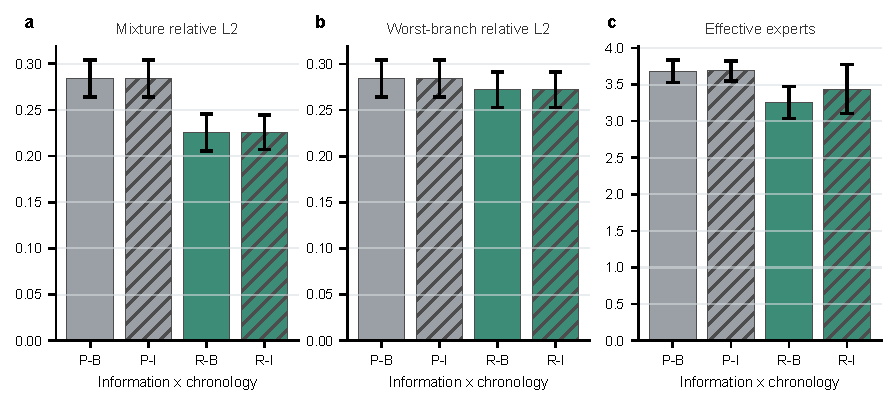
\includegraphics[width=.85\linewidth]{figures/factorial_2x2_bars.pdf}
\caption{Grouped bars for the $2\times2$ factorial experiment (10 paired seeds; mean $\pm$ sample SD). (a) Mixture relative $L_2$; (b) worst complete-branch relative $L_2$; (c) effective experts. Gray denotes physics-only information and green denotes reference guidance; unhatched and hatched bars denote blocked and interleaved updates, respectively. The separation between information sources is much larger than the separation between update chronologies.}
\label{fig:2x2_bars}
\end{figure}

\subsection{Confirmatory composite-protocol comparison: comparable mixture error masks different branch reliability}
\begin{table}[H]
\centering\small
\caption{Primary pre-calibration results on the conservative WENO5 reference (ten paired seeds). Differences are co-adaptive minus staged; $p$ is the exact two-sided sign-flip value.}
\resizebox{\linewidth}{!}{\begin{tabular}{lcccc}
\toprule
Metric & Staged & Co-adaptive & Paired difference [95\% CI] & $p_{\rm exact}$\\
\midrule
Soft-mixture relative $L_2$ & $0.3482\pm0.0170$ & $0.3441\pm0.0126$ & $-0.0041$ [$-0.0155,0.0087$] & 0.5410\\
Worst complete-branch $L_2$ & $0.393\pm0.021$ & $14.50\pm7.27$ & $14.110$ [$9.971,18.477$] & 0.00195\\
Oracle $L_2$ & $0.306\pm0.020$ & $0.278\pm0.014$ & $-0.0281$ [$-0.0404,-0.0165$] & 0.00391\\
Soft-aggregation gain & $0.0339\pm0.0088$ & $0.9055\pm0.0756$ & $0.8716$ [$0.8226,0.9105$] & 0.00195\\
Soft-routing regret & $0.0019\pm0.0005$ & $0.1175\pm0.0903$ & $0.1156$ [$0.0683,0.1731$] & 0.00195\\
Effective experts & $3.706\pm0.217$ & $2.481\pm0.218$ & $-1.225$ [$-1.450,-0.990$] & 0.00195\\
Top-1 / soft error & $1.002\pm0.007$ & $1.085\pm0.082$ & $0.0824$ [$0.0322,0.1241$] & 0.01758\\
$\tau=2$ / soft error & $1.007\pm0.007$ & $2.039\pm0.681$ & $1.0315$ [$0.6471,1.4486$] & 0.00195\\
Delete highest-load / soft error & $1.011\pm0.023$ & $1.402\pm0.183$ & $0.3908$ [$0.2968,0.4996$] & 0.00195\\
\bottomrule
\end{tabular}}
\label{tab:main}
\end{table}
The mean soft-mixture difference is $-0.00413$, but its paired interval crosses zero and the exact test gives $p=0.541$; the data therefore resolve neither protocol as more accurate in aggregate. The worst complete-branch difference is qualitatively different: it is positive on every seed, with mean $14.11$ and 95\% CI $[9.97,18.48]$ (exact $p=0.00195$, Holm-adjusted $p=0.0176$). The co-adaptive directional branch has global $L_2=14.50\pm7.27$, approximately 37 times the staged worst branch of $0.393\pm0.021$. The prespecified directional-shock-region audit in Fig.~\ref{fig:capability_matrix} also shows a large within-region deficit, ruling out the explanation that global error only penalizes local-expert extrapolation. Figure~\ref{fig:burgers_routing} shows the same failure spatially: staged training maintains a structured four-expert partition, whereas co-adaptive argmax routing concentrates strongly on the smooth expert and the directional-branch error exceeds the displayed range over large areas. Because the protocols have different supervision pathways, these results establish a protocol-level contrast, not that joint updating alone caused it.

\begin{figure}[H]
\centering
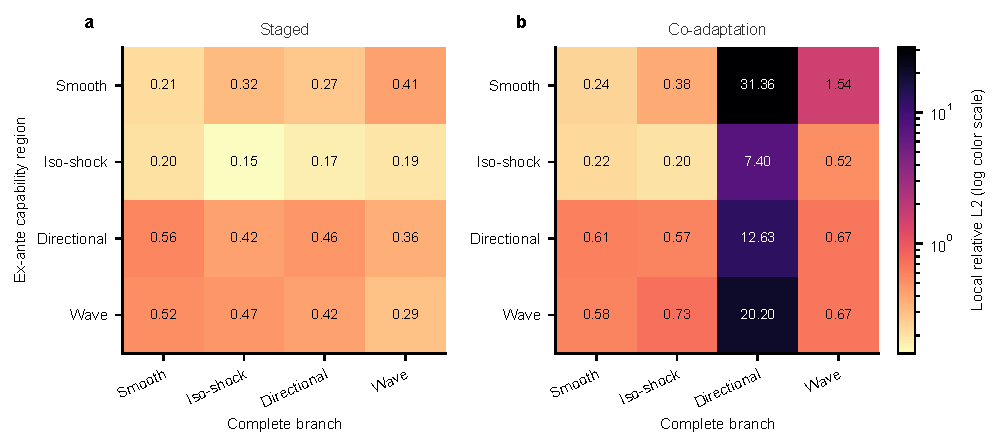
\includegraphics[width=.90\linewidth]{figures/capability_matrix_weno5.pdf}
\caption{Capability-region error matrix on the conservative WENO5 reference. Rows denote ex-ante capability regions and columns denote complete branches. Each cell reports the mean local relative $L_2$ over 10 paired seeds; colors use a logarithmic scale and numbers show the untransformed values. (a) Staged training keeps all cells between approximately $0.2$ and $0.7$. (b) Co-adaptation raises the directional-shock branch to $6.60$--$20.50$ across all regions and also degrades the other branches. Regions are computed from reference derivatives before training and are independent of the learned gate.}
\label{fig:capability_matrix}
\end{figure}

\begin{figure}[H]
\centering
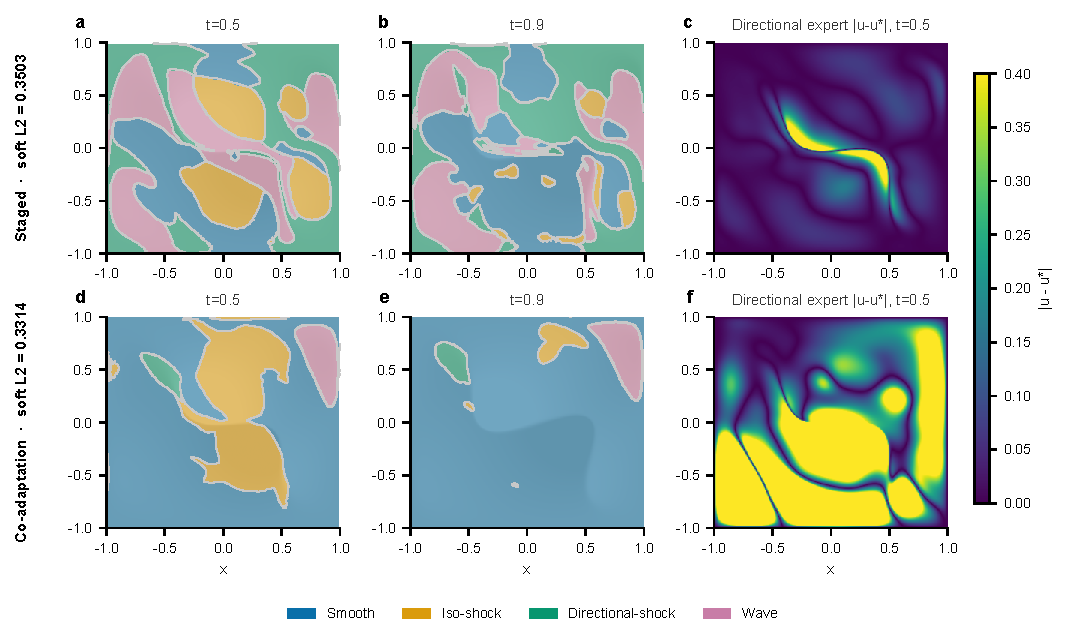
\includegraphics[width=.98\linewidth]{figures/burgers_routing_partition.pdf}
\caption{Routing partitions and directional-branch errors on the full $257^2$ WENO5 visualization grid (seed 43, primary pre-calibration checkpoints). (a--c) Staged and (d--f) co-adaptive. Panels (a,b,d,e) show argmax routing at $t=0.5$ and $t=0.9$, overlaid on the reference field; colors identify Smooth, Iso-shock, Directional-shock, and Wave experts, and light contours mark route boundaries. Panels (c,f) show $|u_{\rm dir}-u^\star|$ at $t=0.5$. Their common Viridis scale is capped at $0.4$ to preserve contrast for the staged panel. Values above $0.4$ are clipped only for display; the reported scalar errors use the separate 344,064-point subset of the $513^2$ reference.}
\label{fig:burgers_routing}
\end{figure}

\begin{figure}[H]
\centering
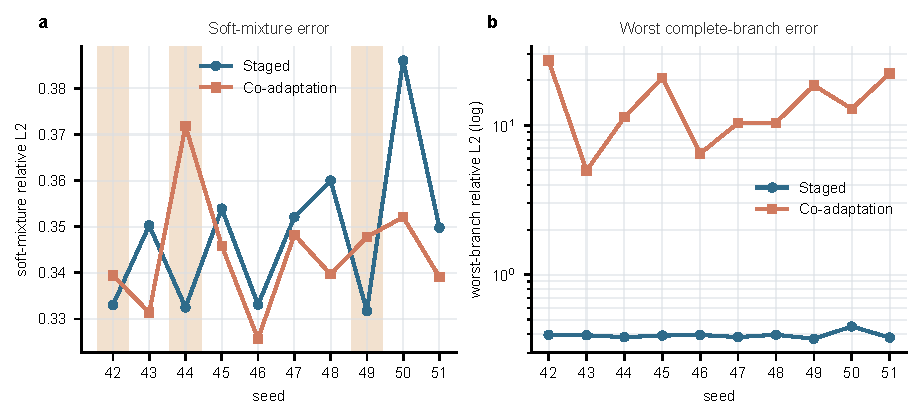
\includegraphics[width=.92\linewidth]{figures/per_seed_paired.pdf}
\caption{Paired-seed results on the conservative WENO5 reference (seeds 42--51, pre-calibration checkpoints). (a) Soft-mixture relative $L_2$; co-adaptation is lower in 7 of 10 pairs, while pale bands mark seeds 42, 44, and 49 where it is higher. (b) Worst complete-branch relative $L_2$ on a logarithmic axis; co-adaptation is more than one order of magnitude higher for every paired seed. Lines connect outcomes across seeds for each protocol and do not represent temporal trajectories.}
\label{fig:per_seed}
\end{figure}

\subsubsection{Mechanism-compatible trajectories}
The seed-42 training trace provides mechanism-level, not population-level, evidence. Figure~\ref{fig:grad_starvation} shows that routing mass progressively concentrates on the smooth and iso-shock experts while the directional-shock mean weight falls to $0.014$. The gradient panel reports the coupled-gradient diagnostic $G_k^{(s)}$ defined above. It therefore demonstrates unequal coupled update signals under the realized mixture objective, not a loss of intrinsic branch approximation capacity.

\begin{figure}[H]
\centering
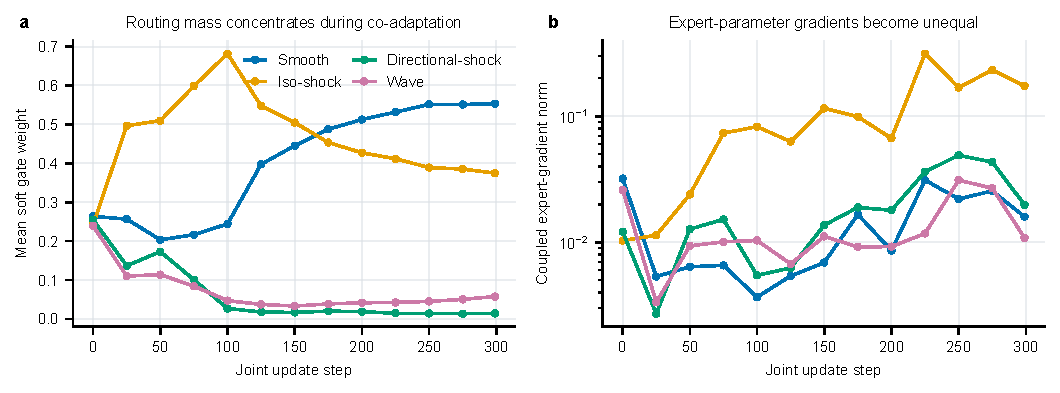
\includegraphics[width=.92\linewidth]{figures/gradient_coupling_trajectory.pdf}
\caption{Gate-weight concentration and coupled expert gradients during co-adaptation (seed 42; fixed 20{,}000-point WENO5 evaluation subset). (a) Domain-mean soft gate weight for the four experts. (b) Coupled expert-parameter gradient norm $G_k^{(s)}=\|\nabla_{\theta_k}\mathcal L_{\rm joint}^{(s)}\|_2$, recorded after backpropagation and before gradient clipping and the Adam update, on a logarithmic axis. The diagnostic contains the gate scaling of the mixture objective and must not be read as an independently evaluated branch-loss gradient. One logged seed is shown, so the figure is mechanistic evidence rather than a sampling estimate.}
\label{fig:grad_starvation}
\end{figure}

Figure~\ref{fig:gap_trajectory} tracks the same seed. Because staged experts are frozen during the gate phase, their capability losses and oracle labels remain fixed by construction. Under co-adaptation, both the median capability gap and the pointwise best-expert labels continue to change. This supports the moving-target interpretation without implying monotonic gap shrinkage or global gate-convergence failure.

\begin{figure}[H]
\centering
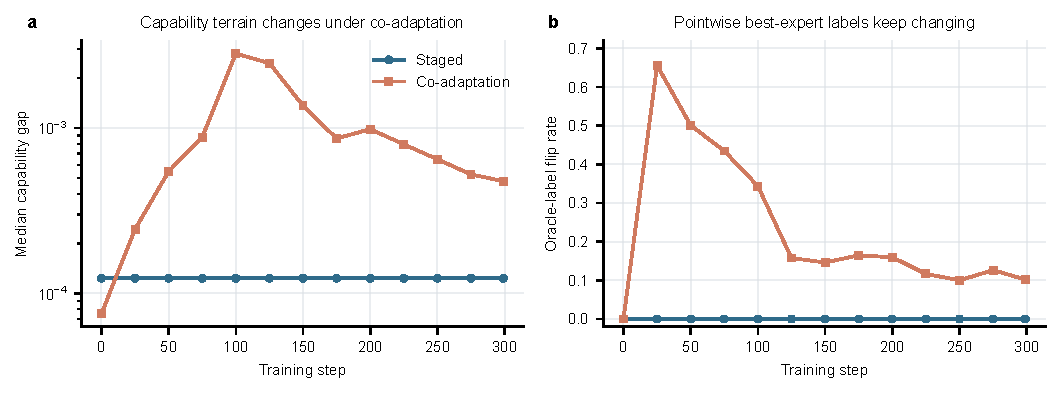
\includegraphics[width=.92\linewidth]{figures/capability_terrain_trajectory.pdf}
\caption{Capability-terrain trajectory under the final protocol (seed 42; fixed 20{,}000-point WENO5 evaluation subset). (a) Median pointwise capability gap $\Delta(z)$ on a logarithmic axis. (b) Fraction of evaluation points whose oracle label changes relative to the previous logged checkpoint. Co-adaptation produces a non-monotone capability terrain and an early flip rate of approximately $0.66$, whereas both quantities remain fixed when staged experts are frozen. The first checkpoint has no previous checkpoint and is plotted with flip rate zero by convention.}
\label{fig:gap_trajectory}
\end{figure}

\subsubsection{Routing-robustness interventions}
The co-adaptive aggregate depends more strongly on the routing regime. Switching to Top-1 routing multiplies its error by $1.085\pm0.082$; flattening the learned weights with $\tau=2$ multiplies it by $2.039\pm0.681$; deleting the highest-load expert multiplies it by $1.402\pm0.183$. The staged ratios are $1.002$, $1.007$, and $1.011$, respectively. All paired intervals in Table~\ref{tab:main} exclude zero. The supported statement is sensitivity to these three prespecified routing interventions, not instability to every perturbation.

\begin{figure}[H]
\centering
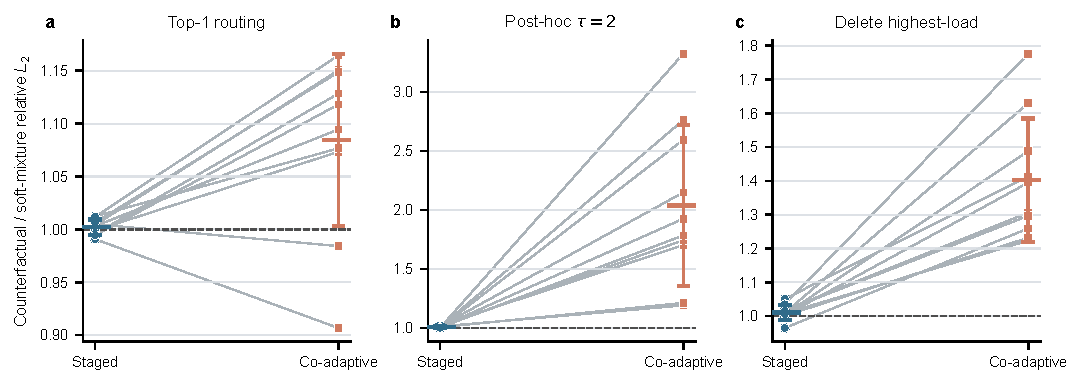
\includegraphics[width=.96\linewidth]{figures/main_counterfactuals.pdf}
\caption{Routing counterfactuals at the primary checkpoint on the same 344,064-point subset of the $513^2$ WENO5 reference (10 paired seeds). Each line joins the same seed across protocols; filled markers and bars show mean $\pm$ sample SD. The ordinate is counterfactual relative $L_2$ divided by the original soft-mixture error, and the dashed line marks one. Top-1 uses argmax routing; $\tau=2$ applies $\widetilde g_k\propto g_k^{1/2}$; ``Delete highest-load'' removes the branch with the largest mean soft load and renormalizes the rest.}
\label{fig:counter}
\end{figure}

\subsection{Exploratory Burgers schedule sweep}
To explore whether forming expert capability before gate introduction is associated with branch health,
we re-evaluated five Burgers training schedules
($f=0\%,25\%,50\%,75\%,100\%$, three seeds) on the conservative WENO5 reference.
Here $f$ denotes 0, 75, 150, 225, or 300 independent updates per expert before the gate is introduced. For $f<100\%$, a cold gate is introduced and experts and gate are then updated jointly for 750 steps. At $f=100\%$, the experts receive all 300 independent updates, the gate receives 180 gate-only updates, and the subsequent 750 steps update only the gate. The schedules therefore differ in both chronology and update allocation; this is an exploratory protocol sweep, not a budget-matched causal estimate of introduction time.
Figure~\ref{fig:gate_intro_burgers} shows that the mixture $L_2$ falls from $0.53$ at $f=0\%$ to $0.36$ at $f=100\%$;
the worst-expert $L_2$ drops from about $5.2$ to $0.40$, more than an order of magnitude;
effective experts rise from $2.5$ to $3.6$ and the minimum load from $0.02$ to $0.13$.
The endpoint contrast is consistent with an association between preformed capability and several audit metrics, but it is not uniformly favorable: the $f=100\%$ schedule has the largest maximum absolute error in this sweep. This countertrend and the protocol differences prevent attribution to timing alone and show why no single scalar metric should certify a schedule.

\begin{figure}[H]
\centering
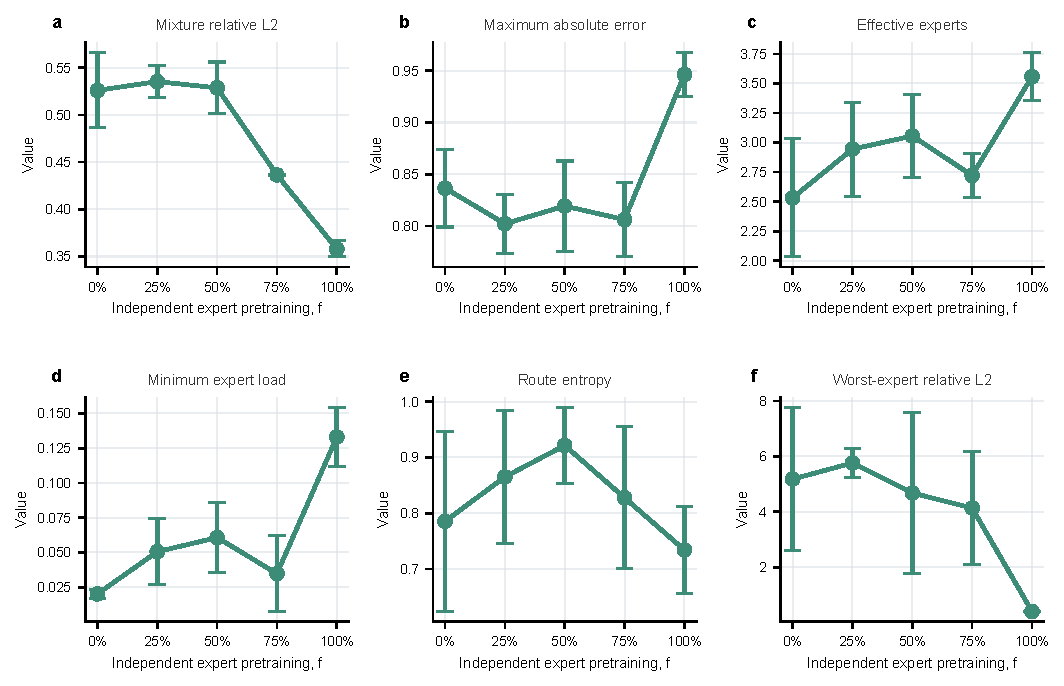
\includegraphics[width=.92\linewidth]{figures/gate_intro_burgers_trajectory.pdf}
\caption{Exploratory Burgers gate-introduction schedule sweep (conservative WENO5 reference, three seeds; mean $\pm$ sample SD).
(a) Mixture relative $L_2$; (b) maximum absolute error; (c) effective experts;
(d) minimum expert load; (e) route entropy; (f) worst-expert $L_2$.
The horizontal axis is the fraction of the 300 independent expert updates completed before gate introduction. Because the $f<100\%$ schedules subsequently update experts and gate jointly whereas $f=100\%$ uses gate-only updates, the curves describe complete training schedules rather than an isolated timing intervention.}
\label{fig:gate_intro_burgers}
\end{figure}

\subsection{Supporting cross-equation and cross-architecture evidence}
For Allen--Cahn, joint refinement from 201 to 401 gives a 0.145\% global difference and a 0.674\% interface difference. The reference describes a moving circular phase boundary. We define the positive-phase interior by $u^\star>0.5$, the negative-phase exterior by $u^\star<-0.5$, and the diffuse interface by $|u^\star|\le0.5$; these reference-defined regions are independent of the learned gate. On this more credible reference, staged/co-adaptive mixture errors are $0.036\pm0.010$/$0.487\pm0.320$. The interface expert's within-specialty error is $0.220\pm0.079$/$3.45\pm1.36$, while its co-adaptive load falls to $0.002\pm0.007$. This is cross-equation evidence for starvation-type degradation\cite{chi2022collapse}. Figure~\ref{fig:allen_bars} summarizes the interface metrics in bar form.

\begin{figure}[H]
\centering
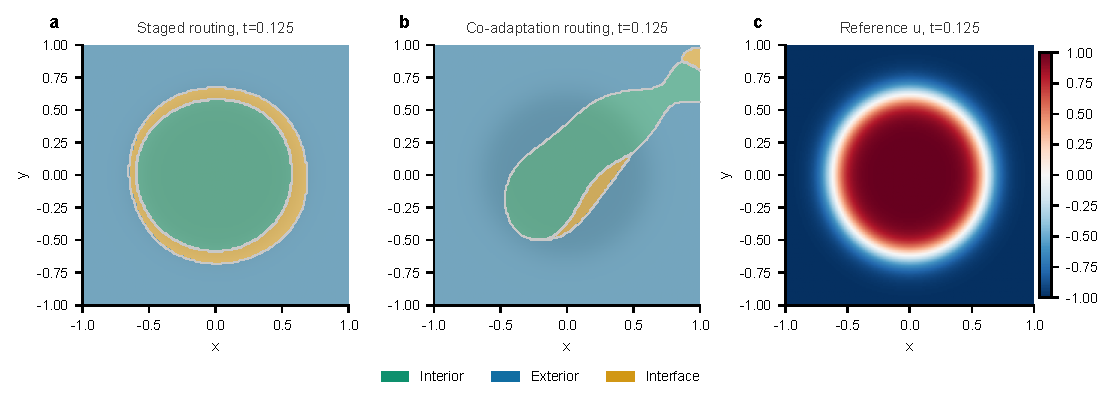
\includegraphics[width=.78\linewidth]{figures/allen_cahn_routing.pdf}
\caption{Allen--Cahn routing at $t=0.125$ for seed 42. (a) Staged and (b) co-adaptive argmax routing; colors identify the interior, exterior, and interface experts. (c) Reference phase field, whose zero-level neighborhood marks the moving circular interface. Staged routing assigns a visible band to the interface expert, whereas co-adaptation nearly removes that band. The region error and load statistics in Fig.~\ref{fig:allen_bars} are computed over the full evaluation grid, not from this single snapshot.}
\label{fig:allen}
\end{figure}

\begin{figure}[H]
\centering
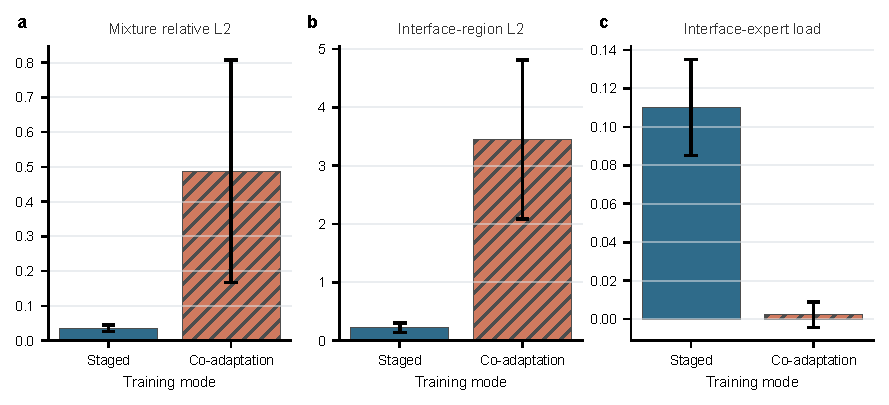
\includegraphics[width=.85\linewidth]{figures/allen_cahn_bars.pdf}
\caption{Allen--Cahn interface metrics (10 paired seeds; mean $\pm$ sample SD). Blue unhatched bars denote staged training and coral hatched bars co-adaptation. (a) Mixture relative $L_2$ over the full domain; (b) interface-expert relative $L_2$ restricted to the prespecified region $|u^\star|\le0.5$; (c) mean soft load of the interface expert. Co-adaptation is worse in (a,b) and assigns almost no routing mass to the interface expert in (c).}
\label{fig:allen_bars}
\end{figure}

APINN controls are re-evaluated on the conservative WENO5 reference. The 186,429-parameter two-subnetwork version gives a soft-mixture error of $0.320\pm0.113$, a worst-subnetwork error of $0.881\pm0.077$, and a Top-1/soft ratio of $1.985\pm0.639$. The official-size two-subnetwork version gives $0.250\pm0.069$, $2.601\pm0.696$, and $3.101\pm0.683$. The four-subnetwork parameter-matched version gives $0.390\pm0.043$, $1.454\pm0.129$, and $1.016\pm0.024$. All three versions exhibit the same aggregate--branch separation. We retain the APINN ratios as supporting cross-architecture evidence and do not rank absolute performance. Figure~\ref{fig:apinn_bars} reports the aggregate, worst-subnetwork, and Top-1/soft metrics for all three versions.

\begin{figure}[H]
\centering
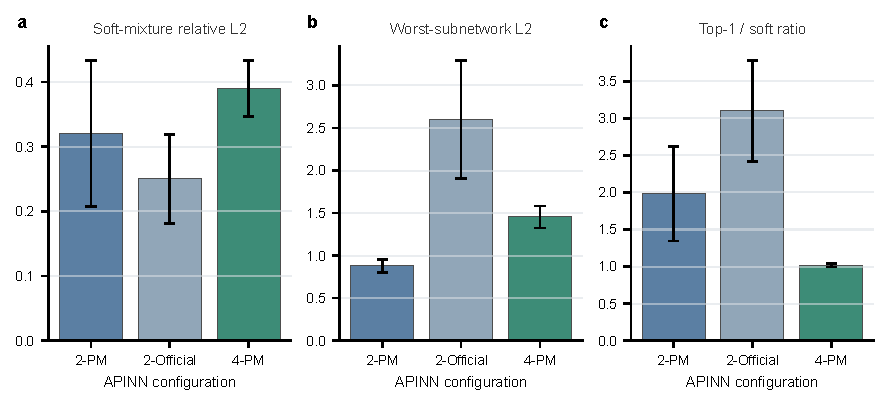
\includegraphics[width=.85\linewidth]{figures/apinn_bars.pdf}
\caption{APINN control metrics on the conservative WENO5 reference (three seeds per configuration; mean $\pm$ sample SD). The configurations are a parameter-matched two-subnetwork model (2-PM), the official-size two-subnetwork model (2-Official), and a parameter-matched four-subnetwork model (4-PM). (a) Soft-mixture relative $L_2$; (b) worst complete-subnetwork relative $L_2$ over the full domain; (c) Top-1/soft error ratio. The comparison is used to test transfer of the aggregate--branch separation across architectures, not to rank their absolute accuracy.}
\label{fig:apinn_bars}
\end{figure}

The exploratory KdV schedule sweep shows more stable oracle coverage and capability gaps when expert capability is formed before routing. Here $f=0\%,25\%,50\%,75\%,100\%$ corresponds to 0, 220, 440, 660, or 880 independent updates per expert before a common 2,200-step joint fine-tuning phase. Only $f=100\%$ additionally receives 400 gate-only steps before joint fine-tuning, so this sweep is also not budget matched. Figure~\ref{fig:kdv_routing} visualizes the routing partition in the $x$--$t$ plane for seed 42, using the interaction window $x\in[-10,8]$. At $f=100\%$, the three experts form a structured partition along the soliton band; over the full test domain their loads are near-uniform ($0.35/0.33/0.32$) with route entropy $0.10$. At $f=0\%$, routing concentrates on the shock expert ($\approx79\%$ of the full space-time domain), and the mixture $L_2$ degrades from $0.025$ to $0.30$. Figure~\ref{fig:kdv_trajectory} summarizes the schedules over three seeds. As $f$ rises from $0\%$ to $25\%$, the mixture $L_2$ drops from $0.32$ to $0.045$ and the worst-expert error from $3.9$ to about $0.8$. At $f=100\%$, the route entropy falls to $0.09$ and the minimum load rises to $0.31$. Because KdV uses an analytic two-soliton solution, this result does not depend on a numerical reference. KdV and Allen--Cahn suggest that the mechanism is not unique to one equation, although confirmatory strength remains concentrated in the ten-seed comparisons.

\begin{figure}[H]
\centering
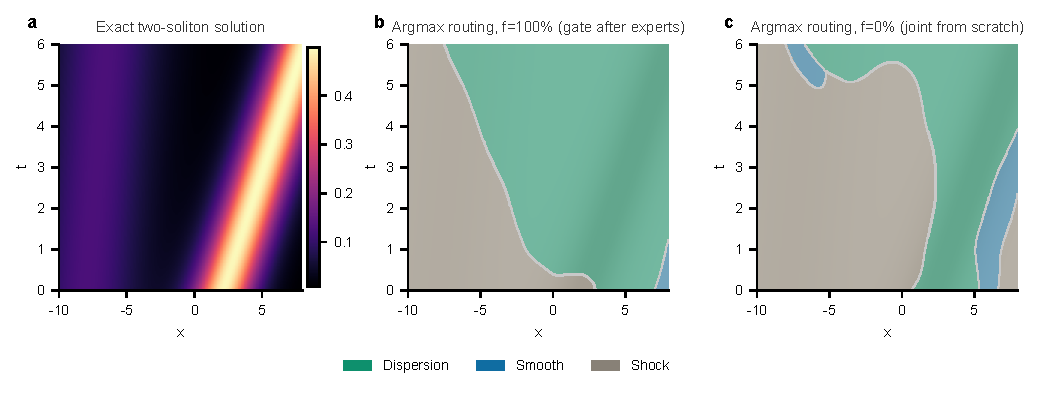
\includegraphics[width=.92\linewidth]{figures/kdv_routing_partition.pdf}
\caption{KdV two-soliton solution and $x$--$t$ routing partitions (seed 42; interaction window $x\in[-10,8]$). (a) Exact solution. (b) $f=100\%$, where the dispersion, smooth, and shock experts form a structured partition along the soliton trajectories. (c) $f=0\%$, where argmax routing concentrates on the shock expert. Colors identify expert identity and are shared across panels (b,c); the exact-solution color scale in (a) represents amplitude rather than routing. The reported loads and errors use the full test domain.}
\label{fig:kdv_routing}
\end{figure}

\begin{figure}[H]
\centering
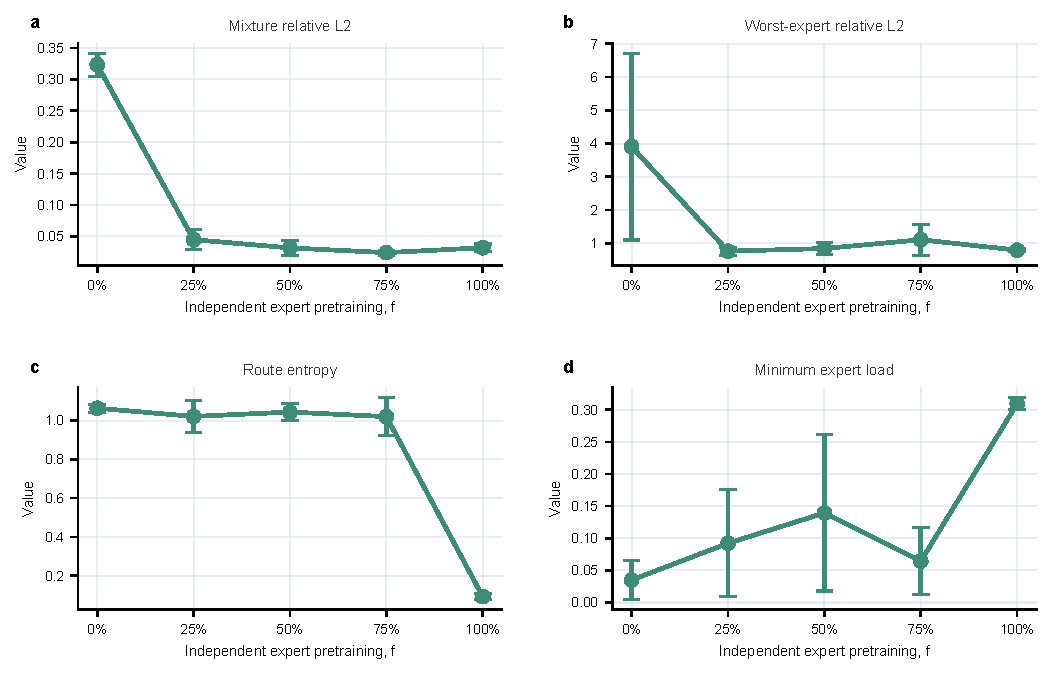
\includegraphics[width=.85\linewidth]{figures/kdv_gate_intro_trajectory.pdf}
\caption{Exploratory KdV gate-introduction schedule sweep (three seeds; mean $\pm$ sample SD). (a) Mixture relative $L_2$; (b) worst complete-expert relative $L_2$; (c) route entropy; (d) minimum mean expert load. The horizontal axis is the fraction of 880 independent expert updates completed before gate introduction. All schedules receive 2,200 joint steps, while only $f=100\%$ receives 400 additional gate-only steps; the trend therefore supports an association but does not isolate introduction time.}
\label{fig:kdv_trajectory}
\end{figure}

\section{Discussion}
\subsection{Supported conclusions}
The mathematics establishes that a mixture-only objective plus gate-only regularization cannot identify branch health. In the actual supervised comparison, the aggregate difference is unresolved, whereas complete-branch degradation, soft-aggregation dependence, routing regret, and the three routing interventions separate the composite protocols consistently. The theorem motivates measuring those quantities but does not prove the optimization cause. Allen--Cahn and KdV provide supporting cross-equation evidence; APINN provides supporting cross-architecture evidence.

\subsection{Boundaries of the claim}
Soft-aggregation gain is not a signed error-cancellation fraction. Mixture error is also not, by itself, statistical overfitting, so we avoid treating ``pseudo-fitting'' as a theorem. Staged training is reference-guided rather than a label-free PINN; its demonstrated benefit is branch auditability under the present protocol, not a universal accuracy advantage. The gate-introduction schedule sweeps use only three seeds and confound introduction time with update allocation, so they are exploratory rather than confirmatory. The branch audit requires a trusted numerical or analytic reference and is presently a benchmark-qualification procedure, not a reference-free online monitor.

\subsection{Limitations and future work}
Our conclusions are limited to the residual soft MoE--PINN architecture, reference-supported training and evaluation, and the tested equations. The three-seed gate-introduction schedules are not part of the main confirmatory conclusions. The non-identifiability theorem is a function-space statement; it does not prove that optimization dynamics must drift along an approximately flat parameter direction, and the single-seed trajectories are only mechanism-compatible. Future work includes (i) a loss-matched factorial design separating direct branch supervision, stop-gradient routing, and joint updating; (ii) breaking non-identifiability with capability regularization; (iii) reference-free proxy audits based on residuals, uncertainty, or certified error estimators; and (iv) hard-routed and pruned deployment studies.

\section{Conclusions}
Soft-mixture prediction, load utilization, and branch health are distinct dimensions of an MoE--PINN. Function-space non-identifiability shows why the first two do not logically imply the third under a mixture-only objective. In the paired Burgers comparison, two composite protocols attain statistically unresolved aggregate accuracy, yet the worst co-adaptive complete branch is approximately 37-fold worse and its aggregate is more sensitive to Top-1 routing, post-hoc flattening, and highest-load deletion. This is a protocol-level reliability contrast, not an isolated causal effect of joint updating. A minimum reference-supported benchmark report should contain same-grid mixture, complete-branch, responsibility-region, and oracle errors; capability-region errors; soft-aggregation gain; routing regret; and routing counterfactuals. These quantities qualify an MoE--PINN before expert removal, hard routing, or gate drift; reference-free proxies remain an open problem.

\section*{Data and code availability}
Machine-readable JSON/CSV source data, training configurations, scripts, and checkpoints are included in the accompanying peer-review archive. A versioned public repository and persistent identifier will be supplied before publication.

\section*{Declaration of competing interest}
The authors declare that they have no known competing financial interests or personal relationships that could have appeared to influence the work reported in this paper.

\begin{thebibliography}{99}\small
\bibitem{raissi2019} M. Raissi, P. Perdikaris, G.E. Karniadakis, Physics-informed neural networks, J. Comput. Phys. 378 (2019) 686--707.
\bibitem{karniadakis2021} G.E. Karniadakis, I.G. Kevrekidis, L. Lu, et al., Physics-informed machine learning, Nat. Rev. Phys. 3 (2021) 422--440.
\bibitem{cuomo2022} S. Cuomo, V.S. Di Cola, F. Giampaolo, et al., Scientific machine learning through PINNs, J. Sci. Comput. 92 (2022) 88.
\bibitem{wang2021grad} S. Wang, Y. Teng, P. Perdikaris, Understanding and mitigating gradient flow pathologies in PINNs, SIAM J. Sci. Comput. 43 (2021) A3055--A3081.
\bibitem{wang2022ntk} S. Wang, X. Yu, P. Perdikaris, When and why PINNs fail to train, J. Comput. Phys. 449 (2022) 110768.
\bibitem{krishnapriyan2021} A. Krishnapriyan, A. Gholami, S. Zhe, et al., Characterizing possible failure modes in PINNs, NeurIPS 34 (2021).
\bibitem{rathore2024} P. Rathore, W. Lei, Z. Frangella, et al., Challenges in training PINNs: a loss landscape perspective, ICML 235 (2024) 42159--42191.
\bibitem{mcclenny2023} L. McClenny, U. Braga-Neto, Self-adaptive physics-informed neural networks, J. Comput. Phys. 474 (2023) 111722.
\bibitem{wu2023} C. Wu, M. Zhu, Q. Tan, et al., Residual-based adaptive sampling for PINNs, Comput. Methods Appl. Mech. Eng. 403 (2023) 115671.
\bibitem{wang2022causal} S. Wang, S. Sankaran, P. Perdikaris, Respecting causality is all you need for training PINNs, arXiv:2203.07404 (2022).
\bibitem{jagtap2020cpinn} A.D. Jagtap, E. Kharazmi, G.E. Karniadakis, Conservative PINNs on discrete domains, Comput. Methods Appl. Mech. Eng. 365 (2020) 113028.
\bibitem{jagtap2020} A.D. Jagtap, G.E. Karniadakis, XPINNs, Commun. Comput. Phys. 28 (2020) 2002--2041.
\bibitem{moseley2023} B. Moseley, A. Markham, T. Nissen-Meyer, FBPINNs, Adv. Comput. Math. 49 (2023) 62.
\bibitem{dolean2024} V. Dolean, A. Heinlein, S. Mishra, B. Moseley, Multilevel domain decomposition-based architectures for PINNs, Comput. Methods Appl. Mech. Eng. 429 (2024) 117116.
\bibitem{hu2023} Z. Hu, A.D. Jagtap, G.E. Karniadakis, K. Kawaguchi, APINNs, Eng. Appl. Artif. Intell. 126 (2023) 107183.
\bibitem{yu2020gradsurgery} T. Yu, S. Kumar, A. Gupta, et al., Gradient surgery for multi-task learning, NeurIPS 33 (2020).
\bibitem{jacobs1991} R.A. Jacobs, M.I. Jordan, S.J. Nowlan, G.E. Hinton, Adaptive mixtures of local experts, Neural Comput. 3 (1991) 79--87.
\bibitem{jordan1994} M.I. Jordan, R.A. Jacobs, Hierarchical mixtures of experts and the EM algorithm, Neural Comput. 6 (1994) 181--214.
\bibitem{krogh1995} A. Krogh, J. Vedelsby, Neural network ensembles, cross validation, and active learning, NeurIPS 7 (1995) 231--238.
\bibitem{shazeer2017} N. Shazeer, N. Mirhoseini, K. Maziarz, et al., Outrageously large neural networks, ICLR (2017).
\bibitem{lepikhin2021} D. Lepikhin, H. Lee, Y. Xu, et al., GShard, ICLR (2021).
\bibitem{fedus2022} W. Fedus, B. Zoph, N. Shazeer, Switch Transformers, J. Mach. Learn. Res. 23 (2022) 1--39.
\bibitem{zoph2022} B. Zoph, I. Bello, S. Kumar, et al., ST-MoE, arXiv:2202.08906 (2022).
\bibitem{zhou2022expertchoice} Y. Zhou, T. Lei, H. Liu, et al., Mixture-of-Experts with expert choice routing, NeurIPS 35 (2022).
\bibitem{puigcerver2024softmoe} J. Puigcerver, C. Riquelme, B. Mustafa, N. Houlsby, From sparse to soft mixtures of experts, ICLR (2024).
\bibitem{chen2022moe} Z. Chen, Y. Deng, Y. Wu, Q. Gu, Y. Li, Towards understanding the mixture-of-experts layer, NeurIPS 35 (2022).
\bibitem{chi2022collapse} Z. Chi, L. Dong, S. Huang, et al., On the representation collapse of sparse mixture of experts, NeurIPS 35 (2022).
\bibitem{li2024merge} P. Li, Z. Zhang, P. Yadav, et al., Merge, then compress, ICLR (2024).
\bibitem{guo2025specialization} H. Guo, H. Lu, G. Nan, et al., Advancing expert specialization for better MoE, NeurIPS 38 (2025).
\bibitem{hinton2015distill} G. Hinton, O. Vinyals, J. Dean, Distilling the knowledge in a neural network, arXiv:1503.02531 (2015).
\bibitem{bischof2021} R. Bischof, M.A. Kraus, Mixture-of-experts-ensemble meta-learning for PINNs, Forum Bauinformatik (2022).
\bibitem{chalapathi2024} N. Chalapathi, Y. Du, A. Krishnapriyan, Scaling physics-informed hard constraints with mixture-of-experts, ICLR (2024).
\bibitem{dan2025moepinn} J. Dan, J. Sun, J. Li, S. Shi, Adaptive optimal selection MoE embedded with PINNs for hyperbolic conservation laws, Commun. Nonlinear Sci. Numer. Simul. 149 (2025) 108936.
\bibitem{shu1988eno} C.-W. Shu, S. Osher, Efficient implementation of essentially non-oscillatory shock-capturing schemes, J. Comput. Phys. 77 (1988) 439--471.
\bibitem{jiang1996weno} G.-S. Jiang, C.-W. Shu, Efficient implementation of weighted ENO schemes, J. Comput. Phys. 126 (1996) 202--228.
\bibitem{gottlieb2001ssp} S. Gottlieb, C.-W. Shu, E. Tadmor, Strong stability-preserving high-order time discretization methods, SIAM Rev. 43 (2001) 89--112.
\bibitem{efron1979} B. Efron, Bootstrap methods: another look at the jackknife, Ann. Stat. 7 (1979) 1--26.
\bibitem{holm1979} S. Holm, A simple sequentially rejective multiple test procedure, Scand. J. Stat. 6 (1979) 65--70.
\end{thebibliography}

\appendix
\section{Notation}
\label{app:notation}

\begin{table}[H]
\centering\small
\caption{Main notation used in the paper.}
\begin{tabular}{ll}
\toprule
Symbol & Meaning\\
\midrule
$z=(x,y,t)$ & space-time point\\
$\mathcal Q$ & space-time domain $\Omega\times(0,T)$\\
$u_{\rm b}$ & shared base network output\\
$e_k$ & residual correction of the $k$th expert\\
$u_k=u_{\rm b}+\alpha e_k$ & complete $k$th single-branch prediction\\
$g_k,\ s_k$ & gating weight and logit\\
$u_{\rm mix}$ & gate-weighted mixture prediction\\
$u^\star$ & reference solution\\
$\delta_k$ & pointwise error of the $k$th branch\\
$E_{\rm mix},\ E_{\rm weighted}$ & mixture and weighted single-branch mean squared error\\
$G_{\rm agg}$ & soft aggregation gain\\
$\ell_k,\ k^\star,\ \Delta$ & local capability loss, oracle branch, capability gap\\
$\varepsilon_{\rm orc}^2,\ \eta,\ \zeta$ & oracle error, mean misrouting weight, non-oracle routing cost\\
\bottomrule
\end{tabular}
\end{table}

\section{Metric definitions}
\label{app:metrics}

Let $\mathcal E$ denote the evaluation point set, $u^\star$ the reference solution, $g_k$ the gating weights, $u_k$ the complete single-branch predictions, and $\ell_k=|u_k-u^\star|^2$. For Burgers, $\mathcal E$ is the 344,064-point subset sampled from the $513^2\times41$ conservative WENO5 reference.

\begin{itemize}[nosep]
  \item \textbf{Mixture relative $L_2$}: $\big(\sum_{z\in\mathcal E}|u_{\rm mix}(z)-u^\star(z)|^2\big)^{1/2}\big/\big(\sum_{z\in\mathcal E}|u^\star(z)|^2\big)^{1/2}$.
  \item \textbf{Single-branch relative $L_2$}: the same with $u_{\rm mix}$ replaced by $u_k$.
  \item \textbf{Responsibility-region absolute RMSE}: $\big(|R_k|^{-1}\sum_{z\in R_k}|u_k(z)-u^\star(z)|^2\big)^{1/2}$, with $R_k=\{z:g_k(z)\ge g_j(z),\ \forall j\}$. The mixture version replaces $u_k$ by $u_{\rm mix}$.
  \item \textbf{Oracle relative $L_2$}: the mixture error with $u_{\rm mix}$ replaced by the pointwise best branch.
  \item \textbf{Soft-routing regret}: $|\mathcal E|^{-1}\sum_{z\in\mathcal E}\big(\sum_k g_k(z)\ell_k(z)-\min_k\ell_k(z)\big)$.
  \item \textbf{Effective experts}: $\exp[-\sum_k\bar g_k\log(\bar g_k+10^{-12})]$, where
  \[\bar g_k=|\mathcal E|^{-1}\sum_{z\in\mathcal E}g_k(z).\]
  \item \textbf{Route entropy and minimum load}:
  \[H_{\rm route}=-|\mathcal E|^{-1}\sum_z\sum_kg_k(z)\log[g_k(z)+10^{-12}],\qquad \min_k\bar g_k.\]
  \item \textbf{Soft-aggregation gain}: $G_{\rm agg}=1-E_{\rm mix}/E_{\rm weighted}$, where $E_{\rm mix}=|\mathcal E|^{-1}\sum_z|u_{\rm mix}-u^\star|^2$ and $E_{\rm weighted}=|\mathcal E|^{-1}\sum_z\sum_k g_k(z)\ell_k(z)$.
  \item \textbf{Top-1, temperature, and deletion ratios}: relative $L_2$ under argmax hard routing, the post-hoc transform $\widetilde g_k(2)\propto g_k^{1/2}$, or deletion of the highest-load expert, divided by the original soft-mixture relative $L_2$.
\end{itemize}

\section{Training configuration}
\label{app:config}

The main model is a residual soft MoE--PINN with 186,727 total parameters.
The base network has input dimension 3 ($x,y,t$), output dimension 1, width 96, depth 5, and tanh activation.
The four experts are smooth (width 48, depth 3), iso-shock (width 96, depth 5),
directional-shock (width 96, depth 5), and wave (width 64, depth 4).
The gate is a local-convolutional context gate of width 64 and depth 3 with learned-router temperature $T_g=0.8$,
16 context neighbors, and a hidden convolution width of 24.

Training protocol: base pretraining for 270 steps (learning rate $10^{-3}$);
independent training of each expert for 300 steps (learning rate $10^{-3}$, 1,800 supervised points per expert);
static-teacher gate training for 300 steps (learning rate $5\times10^{-4}$);
or co-adaptation as 300 joint updates with expert/gate learning rates $10^{-3}$/$5\times10^{-4}$.
The primary checkpoint is saved here. An optional 750-step gate-only calibration is archived but excluded from the primary analysis.
Collocation points: $n_{\rm col}=6000$, $n_{\rm ic}=1200$, and 400 points per boundary face;
loss weights $w_{\rm res}=1$, $w_{\rm ic}=5$, $w_{\rm bc}=2$, and $w_{\rm sup}=8$.
Reference-teacher sharpness is $\beta=8$; the capability-prior exponent is 1.15; the gate balance coefficient is 0.01; and targets are refreshed every ten co-adaptive steps. All experiments use Adam with default moments, Xavier initialization, gradient-norm clipping at one, deterministic seeds 42--51, and the same sampled sets within each paired seed. The recorded environment is Python 3.10.10, PyTorch 2.6.0+cu124, NumPy 2.2.6, and SciPy 1.15.3.

APINN configurations:
\begin{itemize}[nosep]
\item parameter-matched two-subnetwork: shared and subnet widths 143/depth 3; gate width 48/depth 1; 186,429 parameters; scalar binary gate and official XPINN prior with prior temperature 0.32;
\item official-size two-subnetwork: shared width 20/depth 2, subnet width 20/depth 3, gate width 20/depth 1; 3,583 parameters; the same XPINN prior;
\item parameter-matched four-subnetwork: shared and subnet widths 112/depth 3, gate width 48/depth 2; 193,480 parameters; spatial prior.
\end{itemize}
The two-subnetwork models use 10,000 gate-pretraining steps; the four-subnetwork model uses 1,000. All use 8,000 joint steps, gate/train learning rates $10^{-3}$/$8\times10^{-4}$, weight decay $10^{-3}$, $n_{\rm col}=6000$, $n_{\rm ic}=1200$, 400 boundary points per face, and residual/initial/boundary weights 1/10/5.

For Allen--Cahn, $u_t=\Delta u+\epsilon^{-2}(u-u^3)$ on $[-1,1]^2\times[0,0.25]$, $\epsilon=0.08$, $u(x,y,0)=\tanh[(0.8-\sqrt{x^2+y^2})/(\sqrt2\epsilon)]$, and boundary value $-1$. The reference uses exact reaction updates followed by Crank--Nicolson diffusion diagonalized by a discrete sine transform, with a $201^2$ grid and $\Delta t=2\times10^{-4}$; a $401^2$, $10^{-4}$ refinement gives the differences reported in Section 5.4. Three width-96/depth-5 experts represent interior, exterior, and interface behavior; the gate has width 48/depth 3 and $T_g=0.8$. Each expert and the main phase use 1,500 steps.

For KdV, $u_t+6uu_x+u_{xxx}=0$ on $[-20,20]\times[0,6]$. The exact two-soliton solution is $u=2\partial_{xx}\log F$, with $F=1+e^{\eta_1}+e^{\eta_2}+A_{12}e^{\eta_1+\eta_2}$, $\eta_i=k_ix-k_i^3t+\delta_i$, $(k_1,k_2)=(1,0.5)$, $(\delta_1,\delta_2)=(0,4)$, and $A_{12}=[(k_1-k_2)/(k_1+k_2)]^2$. The three experts have widths/depths 96/5, 64/3, and 96/5; the width-32/depth-3 gate uses $T_g=0.9$. The full independent phase is 880 steps per expert, the gate-only phase 400 steps, and joint fine-tuning 2,200 steps; the schedule sweep is not update-budget matched.

\section{Derivations and proof supplement}
\label{app:proofs}

\subsection{Derivation of the gate--expert coupled gradient}

By \eqref{eq:model}, the mixture output depends on the expert parameters $\theta_k$ through
$u_{\rm mix}=u_{\rm b}+\alpha\sum_j g_je_j$, so $\partial u_{\rm mix}/\partial e_k=\alpha g_k$.
The chain rule gives $\nabla_{\theta_k}\mathcal J=(D_{\theta_k}e_k)^*[\alpha g_kq]$.
For the gate logit $s_k$, note that
$\partial g_k/\partial s_k=g_k(1-g_k)/T_g$ and $\partial g_j/\partial s_k=-g_jg_k/T_g$,
hence
\begin{equation}
\frac{\partial u_{\rm mix}}{\partial s_k}
=\frac{\alpha}{T_g}\Big[g_k(1-g_k)e_k-\sum_{j\ne k}g_jg_ke_j\Big]
=\frac{\alpha}{T_g}g_k(e_k-\bar e).
\end{equation}
Substituting $D_{s_k}\mathcal J[\xi]=\langle q,\partial u_{\rm mix}/\partial s_k\,\xi\rangle$ gives \eqref{eq:coupling}.

\subsection{Expansion of the Jensen identity}

Pointwise expansion of the mixture error:
\begin{equation}
\Big|\sum_k g_k\delta_k\Big|^2
=\sum_{i,j}g_ig_j\delta_i\delta_j
=\sum_k g_k|\delta_k|^2
-\frac12\sum_{i,j}g_ig_j|\delta_i-\delta_j|^2,
\end{equation}
where the second step uses
$\sum_{i,j}g_ig_j|\delta_i-\delta_j|^2
=2\sum_k g_k|\delta_k|^2-2\sum_{i,j}g_ig_j\delta_i\delta_j$.
The cross term is nonnegative, so the mixture error does not exceed the weighted single-branch error.

\subsection{Proof of the error bound}

At a fixed point $z$, let $k^\star$ denote the oracle branch. Rewrite the mixture error as
\begin{equation}
u_{\rm mix}-u^\star
=g_{k^\star}(u_{k^\star}-u^\star)+\sum_{j\ne k^\star}g_j(u_j-u^\star).
\end{equation}
Pointwise Jensen gives
$|\sum_kg_k(u_k-u^\star)|^2\le\sum_kg_k|u_k-u^\star|^2$.
Separating the oracle term and using $g_{k^\star}\le1$, then integrating over $\mathcal Q$, yields
$\varepsilon_{\rm mix}^2\le\varepsilon_{\rm orc}^2+\zeta$.
Since $\zeta\le M^2\sum_{j\ne k^\star}g_j=M^2\eta$, the second inequality in \eqref{eq:bound} follows.

\section{Per-seed results}
\label{app:per_seed}

\begin{table}[H]
\centering\scriptsize
\caption{Per-seed main results on the conservative WENO5 reference solution.}
\resizebox{\linewidth}{!}{%
\begin{tabular}{clcccccc}
\toprule
Seed & Mode & Soft-mixture $L_2$ & Worst-branch $L_2$ & Top-1 ratio & $T{=}2$ ratio & Delete-expert ratio & Effective experts\\
\midrule
42 & staged & 0.3330 & 0.3949 & 1.012 & 0.999 & 1.009 & 3.606\\
42 & coadapt & 0.3394 & 27.12 & 1.164 & 3.324 & 1.630 & 2.470\\
43 & staged & 0.3503 & 0.3927 & 0.999 & 1.012 & 1.008 & 3.956\\
43 & coadapt & 0.3314 & 4.968 & 1.073 & 1.190 & 1.223 & 2.587\\
44 & staged & 0.3325 & 0.3814 & 0.991 & 1.021 & 1.051 & 3.646\\
44 & coadapt & 0.3718 & 11.33 & 0.907 & 1.702 & 1.413 & 2.419\\
45 & staged & 0.3539 & 0.3907 & 0.996 & 1.012 & 1.018 & 3.616\\
45 & coadapt & 0.3459 & 20.72 & 1.128 & 2.149 & 1.306 & 2.867\\
46 & staged & 0.3331 & 0.3946 & 0.994 & 1.005 & 1.016 & 3.412\\
46 & coadapt & 0.3257 & 6.470 & 1.118 & 1.212 & 1.297 & 2.681\\
47 & staged & 0.3521 & 0.3816 & 1.003 & 1.008 & 1.001 & 3.925\\
47 & coadapt & 0.3483 & 10.36 & 1.095 & 1.743 & 1.232 & 2.356\\
48 & staged & 0.3600 & 0.3958 & 1.004 & 1.006 & 1.002 & 3.340\\
48 & coadapt & 0.3397 & 10.40 & 1.151 & 1.925 & 1.395 & 2.661\\
49 & staged & 0.3317 & 0.3717 & 1.005 & 1.005 & 1.005 & 3.895\\
49 & coadapt & 0.3478 & 18.51 & 0.984 & 2.762 & 1.488 & 2.129\\
50 & staged & 0.3860 & 0.4495 & 1.006 & 1.002 & 0.965 & 3.798\\
50 & coadapt & 0.3521 & 12.90 & 1.149 & 1.784 & 1.259 & 2.346\\
51 & staged & 0.3498 & 0.3788 & 1.012 & 1.000 & 1.035 & 3.867\\
51 & coadapt & 0.3391 & 22.25 & 1.077 & 2.594 & 1.776 & 2.295\\
\bottomrule
\end{tabular}}
\end{table}

Per-seed data show that co-adaptation attains a higher soft-mixture error on seeds 42, 44, and 49,
whereas its worst-branch error exceeds the staged value on all ten seeds.
The conclusion that co-adaptation is more fragile is therefore not seed-dependent,
while the lower-mixture-error advantage of co-adaptation holds for a majority of seeds rather than universally.

\subsection{APINN per-seed results}

\begin{table}[H]
\centering\scriptsize
\caption{Per-seed APINN results on the conservative WENO5 reference (three seeds per version).}
\begin{tabular}{llccc}
\toprule
Version & Seed & Soft-mixture $L_2$ & Worst-subnetwork $L_2$ & Top-1/soft ratio\\
\midrule
2-sub, parameter-matched & 42 & 0.2644 & 0.968 & 2.223\\
2-sub, parameter-matched & 43 & 0.2460 & 0.824 & 2.470\\
2-sub, parameter-matched & 44 & 0.4508 & 0.850 & 1.262\\
2-sub, official size & 42 & 0.2235 & 2.651 & 2.331\\
2-sub, official size & 43 & 0.3281 & 1.880 & 3.340\\
2-sub, official size & 44 & 0.1988 & 3.270 & 3.632\\
4-sub, parameter-matched & 42 & 0.4403 & 1.576 & 1.022\\
4-sub, parameter-matched & 43 & 0.3662 & 1.468 & 0.989\\
4-sub, parameter-matched & 44 & 0.3638 & 1.319 & 1.037\\
\bottomrule
\end{tabular}
\end{table}

\subsection{Allen--Cahn per-seed results}

\begin{table}[H]
\centering\scriptsize
\caption{Per-seed Allen--Cahn results (seeds 42--51). ``Global branch'' evaluates the complete interface branch over the full domain; ``interface-region'' restricts it to $|u^\star|\le0.5$.}
\begin{tabular}{clcccc}
\toprule
Seed & Mode & Mixture $L_2$ & Global branch $L_2$ & Interface-region $L_2$ & Interface load\\
\midrule
42 & staged & 0.0362 & 1.0103 & 0.1818 & 0.0928\\
42 & coadapt & 0.2275 & 1.2846 & 1.9226 & 0.0220\\
43 & staged & 0.0302 & 0.9221 & 0.1918 & 0.0897\\
43 & coadapt & 0.6549 & 1.6199 & 4.8195 & 0.0006\\
44 & staged & 0.0260 & 1.1223 & 0.2028 & 0.1171\\
44 & coadapt & 0.1728 & 1.4371 & 4.5008 & 0.0000\\
45 & staged & 0.0259 & 1.1141 & 0.2083 & 0.1013\\
45 & coadapt & 1.0352 & 1.5495 & 5.1028 & 0.0000\\
46 & staged & 0.0398 & 1.0580 & 0.2191 & 0.1448\\
46 & coadapt & 0.6854 & 1.4684 & 4.8656 & 0.0004\\
47 & staged & 0.0290 & 0.9945 & 0.2018 & 0.1434\\
47 & coadapt & 0.0400 & 0.6666 & 2.2650 & 0.0000\\
48 & staged & 0.0490 & 1.1107 & 0.2028 & 0.0851\\
48 & coadapt & 0.2733 & 1.0056 & 1.0595 & 0.0000\\
49 & staged & 0.0298 & 1.0639 & 0.1544 & 0.1064\\
49 & coadapt & 0.6859 & 1.3001 & 3.9545 & 0.0000\\
50 & staged & 0.0353 & 1.0926 & 0.1809 & 0.0752\\
50 & coadapt & 0.8619 & 1.2259 & 3.5773 & 0.0000\\
51 & staged & 0.0562 & 1.0847 & 0.4522 & 0.1450\\
51 & coadapt & 0.2361 & 1.5905 & 2.3834 & 0.0000\\
\bottomrule
\end{tabular}
\end{table}

\end{document}
